\documentclass[aspectratio=34]{beamer}

% Remove the gratuituous footer
\setbeamertemplate{footline}{}
\setbeamertemplate{navigation symbols}{}
%\renewcommand{\insertnavigation}[1]{}

\usepackage{graphicx}

%\usepackage{rotating}
\usepackage{algorithm}
\usepackage{algorithmicx}
\usepackage{algpseudocode}
\usepackage{xcolor}
\usepackage{setspace}

\makeatletter
\renewcommand{\ALG@beginalgorithmic}{\scriptsize}
\makeatother

\usepackage{caption}
\usepackage{subcaption}

\DeclareMathOperator{\conv}{conv}
\DeclareMathOperator{\st}{s.t.}
\DeclareMathOperator{\dom}{dom}
\DeclareMathOperator{\im}{im}
\DeclareMathOperator{\Ne}{Ne}
\DeclareMathOperator{\sign}{sign}
\DeclareMathOperator{\Var}{Var}
\DeclareMathOperator{\diag}{diag}
\DeclareMathOperator{\vvec}{vec}

%\graphicspath{{"Learning Matchings/figs/"},{../fig/}}

%\usepackage{beamerthemesplit}

% Make footnotes visible. Stolen from http://tex.stackexchange.com/questions/5852/beamer-footnote-text-collides-with-navigation-symbols
\addtobeamertemplate{footnote}{\vspace{-6pt}\advance\hsize-0.5cm}{\vspace{6pt}}
\makeatletter
% Alternative A: footnote rule
\renewcommand*{\footnoterule}{\kern -3pt \hrule \@width 2in \kern 8.6pt}
% Alternative B: no footnote rule
% \renewcommand*{\footnoterule}{\kern 6pt}
\makeatother

\usepackage[natbibapa]{apacite}

\title{Expanding Compressed Sensing and learning}
\author{Kevin Shi \and Kui Tang}
\institute{Columbia University}

\date{11 Dec. 2015}

\begin{document}

\frame{\titlepage}

% Overall outline
\AtBeginSection[]
{
\begin{frame}<beamer>
\frametitle{Outline}
\tableofcontents[currentsection]
\end{frame}
}

\section{Compressed Learning}

\subsection{Review of Calderblank et. al. 09}

\begin{frame}
\frametitle{Learning Compressively-Sensed Data}
    \begin{itemize}
        \item There exist training data ${(x_i,y_i)} \subset \mathbb{R}^n \times {-1,1}$ where the $x_i$ are $k$-sparse, learn binary classifier $f : \mathcal{X} \rightarrow {-1,1}$.
        \item We observe compressively-sensed measurements ${(Ax_i,y_i)} \subset \mathbb{R}^M \times {-1, 1}$ for a $(2k,\epsilon)$ RIP $m \times n$ matrix $A$.
        \item Two options
        \begin{itemize}
            \item Recover $n$-dimensional sparse vectors, learn classifier in the high dimensional space.
            \item \strong{Learn classifier directly in the compressed space!}
        \end{itemize}
\end{frame}

\begin{frame}
    \frametitle{Support Vector Machine Review}
    
\end{frame}

\begin{frame}
    \frametitle{Compressed Learning Bound}
    $$L_{\cal D}(\widehat{z}_{AS}) \leq L_{\cal D}(w^*) + O(CR^2\epsilon + C\log\frac{1}{\delta} / M)  $$
    \begin{figure}
        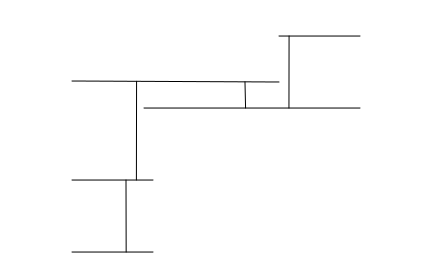
\includegraphics[width=\columnwidth]{bounds_argument_figure.pdf}
    \end{figure}
\end{frame}

\begin{frame}
    \frametitle{RIP for Dot Products}
\end{frame}

\subsection{Extension to Regression}

\begin{frame}
    \frametitle{Support Vector Regression}
\end{frame}

\begin{frame}
    \frametitle{Compressed Learning for Support Vector Machines}
\end{frame}

\subsection{Other Attempted Generalizations}

\begin{frame}
    \frametitle{Attempts to Generalize to other Kernels}
\end{frame}

\begin{frame}
    \frametitle{Attempts to Generalize to Linear Regression}
\end{frame}

\section{Other matrices (Kevin's section)}

\subsection{Overview}
\begin{frame}
    \frametitle{Overview}
\end{frame}

\subsection{Poisson Random Matrices}
\begin{frame}
    \frametitle{Poisson Random Matrices}
\end{frame}

\begin{frame}[t,allowframebreaks]{}
\frametitle{References}

\bibliographystyle{plainnat}
\bibliography{biblio}
\end{frame}


\end{document}

